\documentclass[12pt]{article}
\usepackage{graphicx}
\usepackage[none]{hyphenat}
\usepackage{graphicx}
\usepackage{listings}
\usepackage[english]{babel}
\usepackage{graphicx}
\usepackage{caption} 
\usepackage{booktabs}
\usepackage{array}
\usepackage{amssymb} % for \because
\usepackage{amsmath}   % for having text in math mode
\usepackage{extarrows} % for Row operations arrows
\usepackage{listings}
\lstset{
  frame=single,
  breaklines=true
}
\usepackage{hyperref}
  
%Following 2 lines were added to remove the blank page at the beginning
\usepackage{atbegshi}% http://ctan.org/pkg/atbegshi
\AtBeginDocument{\AtBeginShipoutNext{\AtBeginShipoutDiscard}}


%New macro definitions
\newcommand{\mydet}[1]{\ensuremath{\begin{vmatrix}#1\end{vmatrix}}}
\providecommand{\brak}[1]{\ensuremath{\left(#1\right)}}
\providecommand{\norm}[1]{\left\lVert#1\right\rVert}
\providecommand{\abs}[1]{\left\vert#1\right\vert}
\newcommand{\solution}{\noindent \textbf{Solution: }}
\newcommand{\myvec}[1]{\ensuremath{\begin{pmatrix}#1\end{pmatrix}}}
\let\vec\mathbf


\begin{document}

\begin{center}
\title{\textbf{Conic Sections - Circle}}
\date{\vspace{-5ex}} %Not to print date automatically
\maketitle
\end{center}
\setcounter{page}{1}

\section{10$^{th}$ Maths - Chapter 10}
This is Problem-1 from Exercise 10.2
\begin{enumerate}
\item From a point $\vec{Q}$, the length of the tangent to a circle is $24 cm$ and the distance of $\vec{Q}$ from the centre is $25 cm$. Find the radius of the circle. Draw the circle and the tangents. \\ 
\solution 
Let $\vec{Q}$ be $\vec{Q}\myvec{0 \\ 0}$. Let $\vec{O}$ be the centre of the circle. Let $\vec{R}_1 \text{ and } \vec{R}_2$ be the two points on the circle such that $R_1Q$ and $R_2Q$ are tangents to the circle from the point $\vec{Q}$. Given that,  
\begin{align}
	OQ &= 25, R_1Q = R_2Q = 24 \\ 
	\therefore \vec{O} &= \vec{O}\myvec{25 \\ 0} \\
	r &= OR_1 = \sqrt{OQ^2 - R_1Q^2}  \\
	&= \sqrt{25^2 - 24^2} \\
	&= 7cm
\end{align}
We have to find points $\vec{R}_1 \text{ and } \vec{R}_2$. \\
We know that the equation to the circle is given as
\begin{align}
	\label{eq:circEq1}
	\norm{\vec{x}}^2+2\vec{x}^\top\vec{u}+f = 0 
\end{align}
where
\begin{align}
	\vec{u} &= -\vec{O}  = -\myvec{25 \\ 0}\text{ and } \\
        \label{eq:fRelation}
	f &= \norm{\vec{O}}^2 - r^2 = 576
\end{align}
\begin{align}
	\vec{\Sigma} &= \brak{\vec{Q}+\vec{u}}\brak{\vec{Q}+\vec{u}}^\top - \brak{\norm{\vec{Q}}^2+2\vec{u}^\top\vec{Q}+f}\vec{I}
\end{align}
\begin{align}
	&= \brak{\myvec{0 \\0}-\myvec{25 \\ 0}}\brak{\myvec{0 \\ 0}-\myvec{25 \\0}}^\top - \brak{0-2\myvec{25 & 0}\myvec{0 \\0}+576}\vec{I} \\ 
	&= \myvec{-25 \\0}\myvec{-25 & 0} - \brak{576}\vec{I} \\ 
	&= \myvec{625 & 0 \\ 0 & 0 } - \myvec{576 & 0 \\ 0 & 576} \\ 
        \label{eq:Eq1}
	&= \myvec{49 & 0 \\ 0 & -576 } 
\end{align}
From \eqref{eq:Eq1}, we can deduce Eigen pairs as follow: 
\begin{align}
	\lambda_1 &= 49 , \lambda_2 = -576 \\
	\vec{p_1} &= \myvec{1 \\ 0} , \vec{p_2} = \myvec{0 \\ 1}
\end{align}
Then
\begin{align}
	\vec{n_1} &= \myvec{1 & 0 \\ 0 & 1}\myvec{\sqrt{\abs{\lambda_1}} \\ \sqrt{\abs{\lambda_2}}} = \myvec{7 \\ 24} \\
	\vec{n_2} &= \myvec{1 & 0 \\ 0 & 1}\myvec{\sqrt{\abs{\lambda_1}} \\ -\sqrt{\abs{\lambda_2}}} = \myvec{7 \\ -24}
\end{align}
The points of contact of a tangent on a circle from an external point is given by 
\begin{align}
	\vec{q_{ij}} &= \brak{\pm r \frac{\vec{n_j}}{\norm{\vec{n_j}}}- \vec{u}},  \quad i,j = 1,2 \\
	\vec{q_{i1}} &= \brak{\pm r \frac{\vec{n_1}}{\norm{\vec{n_1}}}- \vec{u}} \\
	&= \brak{\pm \frac{7}{25}\myvec{7 \\ 24}+ \myvec{25 \\ 0}} \\
	&= \brak{\pm \myvec{\frac{49}{25} \\ \frac{168}{25}} + \myvec{25 \\ 0}} \\
	&= \myvec{\frac{674}{25} \\ \frac{168}{25}}, \myvec{\frac{576}{25} \\ -\frac{168}{25}}
\end{align}
\begin{align}
	\vec{q_{i2}} &= \brak{\pm r \frac{\vec{n_2}}{\norm{\vec{n_2}}}- \vec{u}} \\
	&= \brak{\pm \frac{7}{25}\myvec{7 \\ -24}+ \myvec{25 \\ 0}} \\
	&= \brak{\pm \myvec{\frac{49}{25} \\ \frac{-168}{25}} + \myvec{25 \\ 0}} \\
	&= \myvec{\frac{674}{25} \\ \frac{-168}{25}}, \myvec{\frac{576}{25} \\ \frac{168}{25}}  \\
	\therefore \vec{R}_1 &= \vec{q{22}} = \myvec{\frac{576}{25} \\ \frac{168}{25}}, \vec{R}_2 = \vec{q{12}} = \myvec{\frac{576}{25} \\ -\frac{168}{25}}
\end{align}
The figure is as shown in \ref{fig:Fig1}
\begin{figure}[!h]
	\begin{center}
		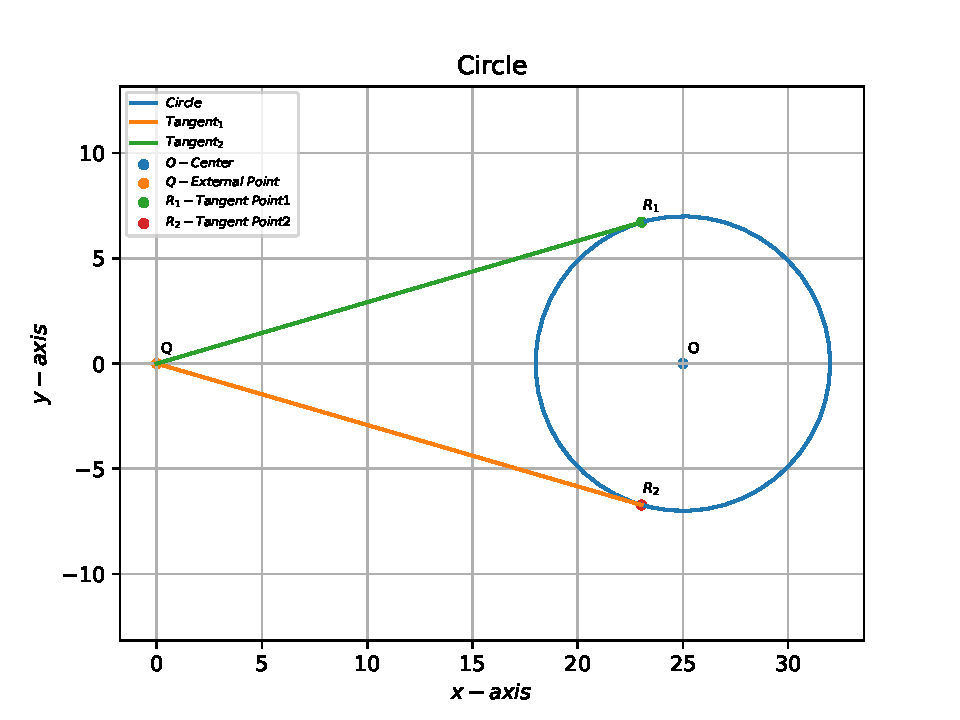
\includegraphics[width=\columnwidth]{./figs/problem1.pdf}
	\end{center}
\caption{}
\label{fig:Fig1}
\end{figure}
\end{enumerate}
\end{document}
